\section{Stand der Forschung}

Die Sicherheit in dem TCP/IP-Protokollfamilie\footnote{Die TCP/IP-Protokollfamilie bezieht sich auf die Aufteilung 
der verschiedenen Ebenen der Diensten und Regel, die in der Netzkommunikation existieren \cite{refbook:SWIS}.} ist 
ein sehr umfangreiches Thema, das sehr viele Facette besitzt. Das Thema beschäftigt sich mit physikalischen 
Koponenten, wie Kabellung und Antennen, und mit abstrakten, wie logische Adressierung oder Übertragung von Signalen.
Die meisten Elementen, die zu Netzwerk gehören, spielen eine wesentliche Rolle für die Gewährleistung
der Netzwerkschutzziele\footnote{Die Netzwerkschutzziele oder IT-Schutzziele sind internationalen Zielen, 
die in dem Netzwerkbereich erreicht werden sollen. Diese Ziele sind Vertraulichkeit, Integrität und 
Authentizität.}. Im folgenden Abschnitt kozentrieren wir uns auf die Gewährleistung der Netzwerkschutzzielen
bei bargeldlosen Zahlungsverfahren. Bevor geben wir eine kurze Einleitung über die Entwicklung von bargeldlosen
Zahlungsmethoden in Deutschland.


\subsection{Chanchen und Risiken vom bargeldlosen Bezahlen}

Die zunehmende Tendenz in Deutschland von bargeldloser Bezahlung erfordert neuen Umgang mit den eigegebenen Daten. 
Eine Studie von 2009 der Deutschen Bundesbank zeigte den rasanten Anstieg von bargeldloser Bezahlung in der
Bundesrepublik seit der Einführung von solchen Zahlungsmethoden \cite{refrep:DBCP}.

\begin{figure}[H]
    \centering{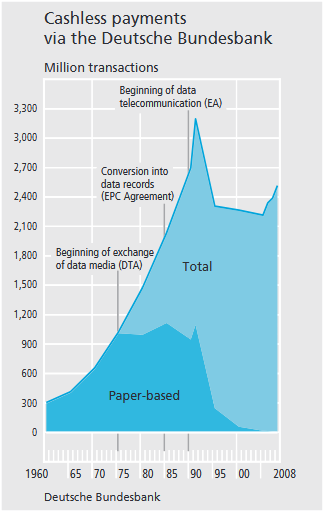
\includegraphics[width=3cm]{Bilder/refrep_DB.png}}
    \caption{Bargeldlose Zahlung über die Deutsche Bundesbank\\ (Bundesbank, 2009, S.52)}
    \label{fig:refrep_DB}
\end{figure}


Laut einer Statistik des Handelsforschungsinstituts EHI von 2019 \cite{refart:KSDL} bezahlen 48,6\% 
der deutschen ihre Waren mit Karte, wohingegen nur noch 46,9\% der deutschen den klassischen 
Weg über Bargeld gehen. Auch das kontaklose Bezahlen, bei dem kleine Beträge nicht einmal mit einer 
PIN bestätigt werden müssen, nimmt immer weiter zu. Doch gerade bei dieser Variante ist es sehr einfach
im Namen eines anderen zu bezahlen, was eine Sicherheitsrisiko darstellt. Diese Tendenz wurde auch
von \cite{refart:TDMP} in seiner Studie beobachtet, bei der er die meist verbreiteten Zahlungsarten
in verschidenen Regionen dieser Welt vergleicht. 


Immer wenn mit Karte bezahlt wird, gehen die Kunden davon aus, dass die Zahlungsabwicklung sicher ist. 
Wie sicher ist das bargeldlose Zahlen heutzutage wirklich? 


\subsection{IT-Schutzziele vom bargeldlosen Zahlungsverfahren}


Vertraulichkeit ist die erste und wichtigste Voraussetzung, das ein solches Zahlungssystem erfüllen muss, 
um neue potenzielle Kunden zu gewinnen. Unter diesem Begriff Vertraulichkeit verstehen wir, dass es keine 
unautorisierte Informtionsgewinnung gibt \cite{refbook:SWIS}.
%Unter diesem Begriff soll ein System nur auf autorisierte Informationen zugreifen. 
In dieser Hinsicht ist die Entwicklung einer Click-and-Buy-Automat so zu konzipieren, dass sie einen sicheren
Umgang mit den Kundendaten anbietet. Die Interaktion zwischen einem Kunden und systemkritischen Mechanismen 
wurde von \cite{refart:HARE} so dargestellt:

\vfill
\begin{figure}[htb]
    \centering{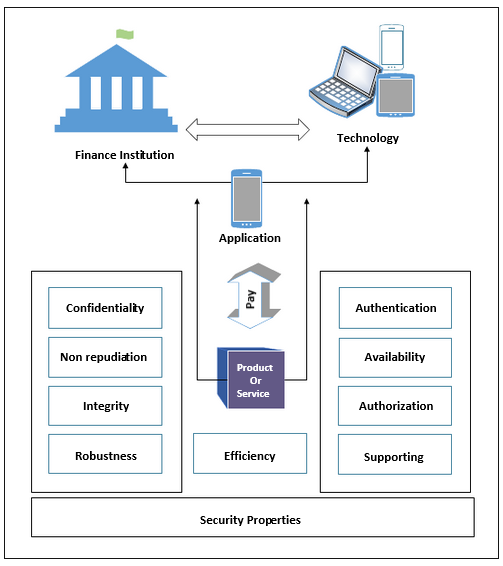
\includegraphics[width=5cm]{Bilder/refark_HARE.png}}
    \caption{Sicherheitseigenschaften von digitalen Zahlungsmethode (Hassan et al. 2020, S8)}
    \label{fig:refark_HARE}
\end{figure}
\vfill

\cite{refart:JTAS} beschreibt didaktisch ein Zahlungsverfahren, dass die Vertraulichkeit gewährleisten kann.
Dieses findet in verschieden 2 getrennte Schritten statt.

Im ersten Schritt, sendet der Nutzer seinen Namen, generiert einen Sitzungsschlüssel und sendet eine Anfrage für
eine Transaktion. Diese Anfrage wird daraufhin an den Händler geschickt, der diese wiederrum bearbeitet. Nachdem 
das abgeschlossen wurde, sendet der Händler seine Antwort an das Bezahlgerät, das wiederrum die Antwort an den Nutzer
weiterleitet. 

Im zweiten Schritt wird die Bezahl Anfrage an das Bezahlgerät gesendet, die unter anderem den Preis und die Uhrzeit enthält.
Das Bezahlgerät leitet die empfangene Nachricht an den Händler weiter. Dieser empfängt die Daten und prüft auf
Aktualität der Daten. Wenn dieser Test erfolgreich ist, wird wieder eine Nachricht an das Bezahlgerät geschickt. 
Dieses schickt die Daten dann wiederrum an die Bank, welche überprüft, ob das Geld von dem Konto abgebucht werden
kann oder nicht. Wenn das geprüft wurde, wird eine Nachricht an das Bezahlgerät gesendet, in der steht, dass das 
Geld abgebucht wurde. 

Besonders wichtig ist, dass bei jeder Kommunikation die Daten kryptographisch verschlüsselt werden, sodass es einem 
potenziellen Angreifer nicht möglich ist, Daten zu ändern oder zu entschlüsseln. In der Folgenden Abbildung wird
da oben genannten Verfahren dargestellt:

\begin{figure}[H]
    \centering{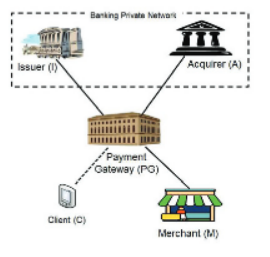
\includegraphics[width=6cm]{Bilder/refart_JTAS_1.png}}
    \caption{Abbildung des Zahlungsverahren \cite{refart:JTAS}}
    \label{fig:refart:JTAS}
\end{figure}

Das folgende Sequenzdiagramm\footnote{Ein Sequenzdiagramm ist ein Verhaltensdiagramm, welches eine Interaktion
im Sinne der Unified Modeling Language (UML) grafisch darstellt \cite{refbook:IASE}.} stellt den 
Nachrichtenaustausch zwischen den Elemeten dieser Zahlungsmethode dar:

\vfill
\begin{figure}[H]
    \centering{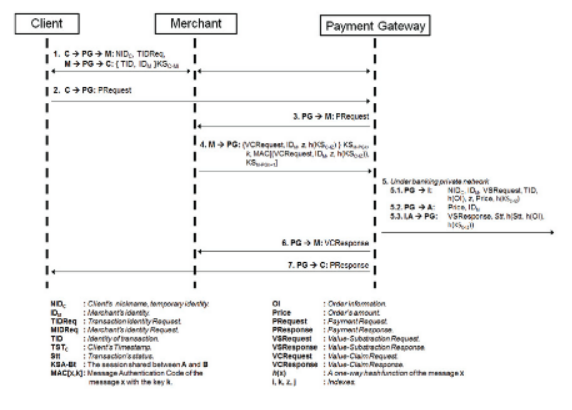
\includegraphics[width=8cm]{Bilder/refart_JTAS_2.png}}
    \caption{Nachrichtenflussaustausch \cite{refart:JTAS}}
    \label{fig:refart:JTAS_2}
\end{figure}

Zudem sollten die weiteren Schutzziele der IT-Sicherheit: Integrität und Authentizität berücksichtigt werden, 
sodass die Zahlungsystemen einwandfrei und sicher funktionieren \cite{refip:GMPS}. Eine Zahlungsmethode, bei der 
alle Vorraussetzungen erfüllt werden, kann in der Lage sein, das Vertrauen und die Akzeptanz von den Nutzenden 
zu bekommen \cite{refart:HARE}. Besonders im deutschen Markt, spielen die oben genannten Schutzziele eine 
wesentliche Rolle für die Akzeptanz irgendwelchen neues Systemens \cite{refip:DKAM}.

Da es um einen dynamischen und breiten Bereich geht, bei dem es sehr schnell zu Änderungen kommen kann, 
besonders bei den Angriffstechniken, müssen die dazu gehörige Technologie stets weiterentwickelt und 
angepasst werden \cite{refip:NYRS}, um Vertraulichkeitsverlust seitens der Kunden zu vermeiden. 
Da die Vertraulichkeit noch nicht zu 100 Prozent gewähleistet werden kann, verweigern viele Kunden
das bargeldlose Bezahlen.

Viele Studien befassen sich mit den verschiedenen Aspekten der Sicherheit bei bargeldlosen Zahlungsmethoden.
Da die Literatur dieses Forschungsfeldes sehr umfangreich ist und da dieses Thema eine breite Vielfältigkeit 
besitzt \cite{refip:GMPS}, sollen hier zwei dieser Technologien in Bezug auf Angriffstechniken und
Gegenmaßnahmen genauer betrachtet werden: drahtlose Verbindungen und Smartcards.

